%-----------------------------------------------------------------
% BEAMER BODY
% !TEX root = ./../main.tex
%-----------------------------------------------------------------
\frame{\maketitle}

% \AtBeginSection[]{% Print an outline at the beginning of sections
% \begin{frame}<beamer>
% 	\frametitle{Outline for Section \thesection}
% 	\tableofcontents[currentsection]
% \end{frame}}

% \AtBeginSection[]{% Print an outline at the beginning of sections
\begin{frame}<beamer>
	% \frametitle{Outline for Section \thesection}
	\frametitle{Outline}
	\tableofcontents%[currentsection]
\end{frame}
% }

%-----------------------------------------------------------------
\section{Introduction}
\begin{darkframes}
	\begin{frame}
		\huge Introduction
	\end{frame}
\end{darkframes}

%---------------------------------
\subsection{Objectives}
\begin{frame}[label=intro-motivation]{Background and motivation}
	% \framesubtitle{Lewis Carroll}
	For the North Atlantic (N.~Atl.) and Northeast Pacific (E.~Pac.) basin, it has been shown \cite{Corral2010} that the probability distribution of the so-called power-dissipation index ($PDI$, a rough estimation of released energy) is affected by the annual and basin-wide averaged sea surface temperature (SST), displacing towards more extreme values on warm years (high-SST).

	\medskip
	As the $PDI$ integrates (cubic) wind speed over tropical-cyclone (TC) lifetime, it is an open question where the $PDI$ increase comes from (higher speed, longer lifetime, or both).
\end{frame}

\begin{frame}[label=intro-objectives]{Objectives}
	\begin{itemize}
		\item Describe the influence of SST on tropical-cyclones occurrences.
		\item Understand the displacement towards more extreme $PDI$ values on warm years (high-SST).
		\item Develop a statistical method to compare the joint distributions of the two populations (low-SST and high-SST).
	\end{itemize}
	% \begin{block}{Practical objectives}
	% 	\begin{itemize}
	% 		\item asd
	% 	\end{itemize}
	% \end{block}

	% \begin{block}{Statistical objective}

	% \end{block}
\end{frame}

%---------------------------------
\subsection{Tropical-cyclones}
\begin{frame}[label=intro-tc]{Tropical-cyclones}
	To characterise a TC one needs to define a physically relevant measure of released energy. The released energy of each TC is summarised as
	\begin{align}\label{eq:pdi}
		PDI = \sum_{t} v_{t}^{3} \Delta t .
	\end{align}
	\begin{itemize}
		\item The raw hurricane best track data (HURDAT2) is provided by the National Hurricane Center.
		\item We limit this study to the satellite era (1966--2016).
	\end{itemize}

	\medskip
	Higher SSTs $\Leftrightarrow$ increased water vapour in the lower troposphere~\cite{Trenberth2005} $\Rightarrow$ separation of years by SST.

\end{frame}

\begin{frame}[label=intro-tc]{Separation by SST}
	Then, the hurricane observational data is classified into occurrences in low-SST and high-SST years depending on whether they are lower or greater than
	\begin{align}
		\ev{\text{SST}} = \sum_{y \in Y} \frac{\text{SST}(y)}{Y} ,
	\end{align}
	where $\text{SST}(y)$ is the mean SST of the year $y$, and $Y$ is the total number of years studied.
	\begin{itemize}
		\item The SST data (HadISST1) is provided by the Met Office Hadley Centre.
	\end{itemize}
\end{frame}

\begin{frame}[label=intro-tc]{Data overview}
	% In \Cref{fig:full-map} we can see a map showing all the storms analysed for both basins (N.~Atl. and E.~Pac.), already divided by SST class, and the spatial window for the $\ev{\text{SST}}$ calculation highlighted in green.
	\begin{figure}[H]
		\centering
		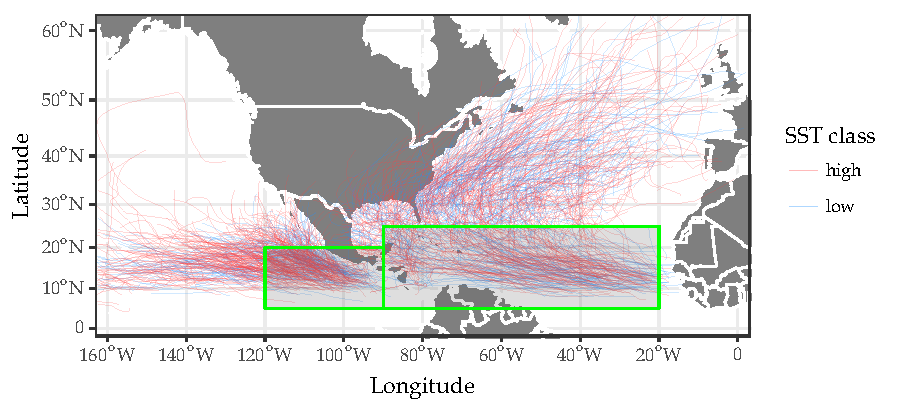
\includegraphics[width=\textwidth]{images/full-map}
		\caption{Tropical-cyclones best tracks for the North Atlantic and Northeast Pacific Oceans}
		\label{fig:full-map}
	\end{figure}

\end{frame}

\begin{frame}[label=intro-tc]{Data package}
	Unified data sets for the N.~Atl. and E.~Pac. basins are available in a R package called \texttt{HurdatHadISSTData} \cite{o:gitlab-data-repo}.
	% \begin{lstlisting}
	% library(devtools)
	% install_git("https://gitlab.com/aldomann/hurdat-hadisst-data.git")
	% \end{lstlisting}

	\medskip
	The data sets in the \texttt{HurdatHadISSTData} package are:
	\begin{itemize}
		\item \texttt{tc.pdi.natl} -- Data set for the North Atlantic basin.
		\item \texttt{tc.pdi.epac} -- Data set for the Northeast Pacific basin.
		\item \texttt{tc.pdi.all} -- Data set for both basins.
	\end{itemize}

	\begin{table}[H]
		\centering
		\ttfamily
		\resizebox{\textwidth}{!}{%
		\begin{tabular}{r r r r r r r r r r r r r}
			\toprule
			\toprule
			storm.id & storm.name & n.obs & storm.duration &    storm.pdi & max.wind & mean.wind & mean.sq.wind & storm.year & basin &   sst & sst.norm & sst.class \\
			<chr>    & <chr>      & <int> &          <dbl> &        <dbl> &    <int> &     <dbl> &        <dbl> &      <int> & <chr> & <dbl> &    <dbl> &     <chr> \\
			\midrule
			AL011966 & ALMA       &    42 &            252 &  34632626747 &      110 &      56.4 &        3750  &       1966 & NATL  &  27.6 &    0.998 &       low \\
			AL021966 & BECKY      &     9 &             54 &   3413930334 &       65 &      46.1 &        2353. &       1966 & NATL  &  27.6 &    0.998 &       low \\
			AL031966 & CELIA      &    36 &            216 &   7839872104 &       70 &      35.4 &        1488. &       1966 & NATL  &  27.6 &    0.998 &       low \\
			AL041966 & DOROTHY    &    37 &            222 &  21340832518 &       75 &      54.9 &        3211. &       1966 & NATL  &  27.6 &    0.998 &       low \\
			AL051966 & ELLA       &    26 &            156 &   4646503652 &       45 &      37.7 &        1487. &       1966 & NATL  &  27.6 &    0.998 &       low \\
			AL061966 & FAITH      &    69 &            414 & 120569417711 &      110 &      79.0 &        6722. &       1966 & NATL  &  27.6 &    0.998 &       low \\
			\bottomrule
		\end{tabular}}
		\caption{Excerpt of the North Atlantic data set}
		\label{hd:unified-dataset-head}
	\end{table}

\end{frame}

\begin{frame}{Data visualisation}
	\begin{onlyenv}<1>
		\begin{figure}[H]
			\centering
			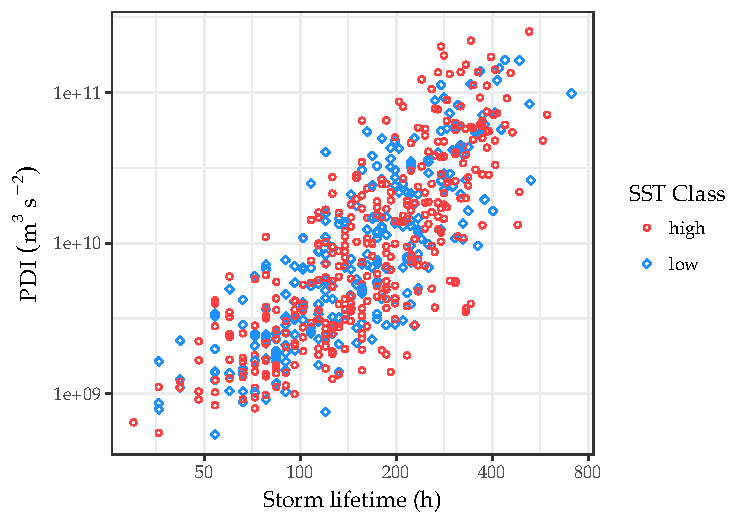
\includegraphics[width=0.8\textwidth]{images/natl-bvln}
			\caption{Joint distribution $f(PDI, \text{lifetime})$ of the hurricane observations for the North Atlantic basin}
			\label{fig:natl-bvln}
		\end{figure}
	\end{onlyenv}
\end{frame}

%---------------------------------
\subsection{Hypothesis}
\begin{frame}[label=intro-hypothesis, allowframebreaks]{Hypothesis}
% \end{frame}
% \framebreak
% \begin{frame}{Hypothesis}
	\begin{onlyenv}<1>
		\begin{block}{Hypothesis statement}
			That $\text{SST}$ does not directly affect the maximum wind speed of a TC: storms of equal lifetime should, in theory, have the same wind speed and $PDI$, and have the same joint distribution:
			\begin{align}\label{eq:hypothesis}
				f(Y \mid X = x)_{\text{low}} = f(Y \mid X = x)_{\text{high}} .
			\end{align}
		\end{block}

		The physical reasoning behind this is that once the cyclone is activated, the wind speed should not depend on its underlying $\text{SST}$.
	\end{onlyenv}
\end{frame}

%-----------------------------------------------------------------
\section{Regression analysis}
\begin{darkframes}
	\begin{frame}
		\huge Regression analysis using resampling methods
	\end{frame}
\end{darkframes}

%---------------------------------
\subsection{Comparing two populations}
\begin{frame}[label=intro-objectives]{Linear regression}
	\framesubtitle{Description of the populations}
	\begin{onlyenv}<1>
		\begin{align}\label{eq:lm-model}
			Y = \beta_{0} + \beta_{1} X + \epsilon.
		\end{align}
		Regression coefficient estimates:
		\footnotesize
	    \begin{align*}
		    \begin{aligned}
		    	\hat{\beta}_{0} &= \bar{y} - \hat{\beta}_{1} \bar{x}, \\
		    	\hat{\beta}_{1} &= \frac{\sum_{i=1}^{n} \qty(x_{i} - \bar{x}) \qty(y_{i} - \bar{y})}{\sum_{i=1}^{n} \qty(x_{i} - \bar{x})^{2}},
		    \end{aligned}
			\qquad &
			\begin{aligned}
				\se{\hat{\beta}_{0}} &= \sqrt{ \sigma^{2} \qty(\frac{1}{n} + \frac{ \bar{x}^{2} }{ \sum_{i=1}^{n} \qty(x_{i} - \bar{x})^{2} } ) },
				\\
				\se{\hat{\beta}_{1}} &= \sqrt{ \frac{ \sigma^{2} }{ \sum_{i=1}^{n} \qty(x_{i} - \bar{x})^{2} } }.
			\end{aligned}
		\end{align*}

		\begin{align*}
			R^{2} = 1 - \frac{\text{RSS}}{\text{TSS}}
				  = 1 - \frac{\sum_{i=1}^{n} \qty(y_{i} - \hat{y}_{i})^{2}}{\sum_{i=1}^{n} \qty(y_{i} - \bar{y}_{i})^{2}}
			\qc \quad
			% \begin{align}
			\hat{\sigma} = \sqrt{\frac{\text{RSS}}{n - 2}} = \sqrt{\frac{\sum_{i=1}^{n} \qty(y_{i} - \hat{y}_{i})^{2}}{n-1}}.
			% \end{align}
		\end{align*}
	\end{onlyenv}

	\begin{onlyenv}<2>
 		\begin{figure}[H]
 			\centering
 			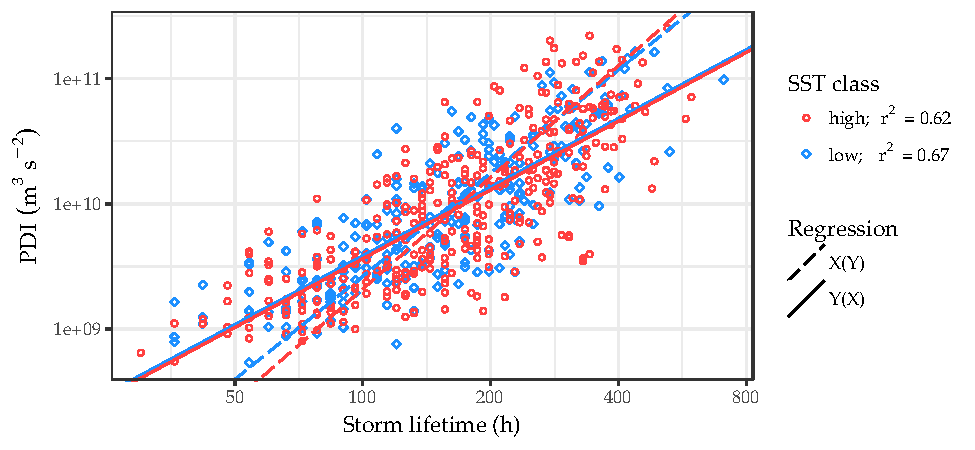
\includegraphics[width=\textwidth]{images/scatterplot-natl}
 			\caption{Scatterplot of the joint distribution and regression analysis for the $PDI$ and lifetime of storms for the North Atlantic basin}
 			\label{fig:natl-scatterplot}
 		\end{figure}
	\end{onlyenv}

	\begin{onlyenv}<3>
		\begin{figure}[H]
			\centering
			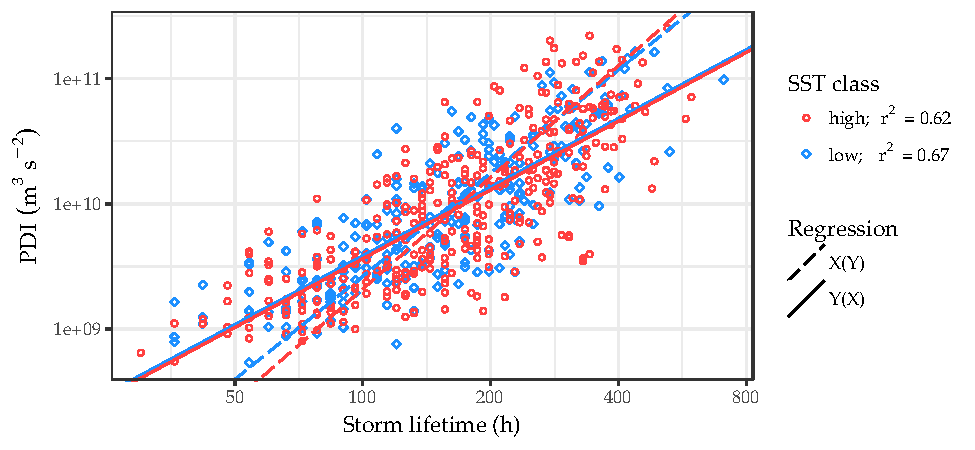
\includegraphics[width=0.7\textwidth]{images/scatterplot-natl}
			% \caption{Scatterplot of the joint distribution and regression analysis for the $PDI$ and lifetime of storms for the North Atlantic basin}
			% \label{fig:natl-scatterplot}
		\end{figure}

 		\begin{table}[H]
 			\centering
 			\resizebox{0.8\textwidth}{!}{%
 			\begin{tabular}{cccccc}
 				\toprule
 				\toprule
 				$X$ & $Y$ & SST class & $\hat{\beta}_{0}$ & $\hat{\beta}_{1}$ & $R^{2}$ \\
 				\midrule
 				% \cmidrule(l){2-5}
 				\multirow{2}{*}{lifetime} & \multirow{2}{*}{$PDI$}
 				 & Low  & \num{-1.44 \pm 0.16} & \num{0.37 \pm 0.02} & \num{0.67} \\ % \pm 0.05} \\
 				&& High & \num{-1.14 \pm 0.14} & \num{0.34 \pm 0.01} & \num{0.62} \\ % \pm 0.04} \\
 				\midrule
 				\multirow{2}{*}{$PDI$} & \multirow{2}{*}{lifetime}
 				 & Low  & \num{ 5.94 \pm 0.18} & \num{1.82 \pm 0.08} & \num{0.67} \\ % \pm 0.05} \\
 				&& High & \num{ 5.91 \pm 0.17} & \num{1.83 \pm 0.08} & \num{0.62} \\ % \pm 0.04} \\
 				\bottomrule
 			\end{tabular}}
 			\caption{Linear regression coefficients obtained performing OLS on the North Atlantic basin data}
 			\label{tab:natl-ols-coefs}
 		\end{table}
	\end{onlyenv}
\end{frame}

\begin{frame}{Comparing the two populations}
	It seems straightforward to compare the coefficient estimates directly:
	{\footnotesize
	\begin{align}
		T^{(1)} = \abs{\hat{\beta}_{0,h} - \hat{\beta}_{0,l}}
		\qc
		T^{(2)} = \abs{\hat{\beta}_{1,h} - \hat{\beta}_{1,l}}
		\qc
		T^{(3)} = \abs{ R^{2}_{h} - R^{2}_{l} } \label{eq:h0-stat-simple} .
	\end{align}
	}%

	\textcite{Polko-Zajac2016} proposes alternative statistics that not only consider the nominal value of the coefficient estimates, but take into account their standard errors as well:
	{\footnotesize
	\begin{align}
		T^{(4)} = \frac{\abs{\hat{\beta}_{0,h} - \hat{\beta}_{0,l}}}{\se{\hat{\beta}_{0,h} - \hat{\beta}_{0,l}}}
		\qc
		T^{(5)} = \frac{\abs{\hat{\beta}_{1,h} - \hat{\beta}_{1,l}}}{\se{\hat{\beta}_{1,h} - \hat{\beta}_{1,l}}}
		\qc
		T^{(6)} = T^{(4)} + T^{(5)} \label{eq:h0-stat-polko} .
	\end{align}
	}%
\end{frame}

\begin{frame}[label=intro-objectives]{Assumptions for the model}
	% \framesubtitle{Lewis Carroll}
	\begin{onlyenv}<1>
		\begin{itemize}
			\item Normality of the residuals.
			\item Homoscedasticity of the residuals.
			\item Independence of the residuals.
		\end{itemize}
		The standard errors, confidence intervals, and hypothesis tests associated with the linear model rely upon these being true.
	\end{onlyenv}

	\begin{onlyenv}<2>
		Diagnostic plots:
		\begin{itemize}
			\item Q-Q plot of the residuals.
			\item Residuals vs fitted values plot.
		\end{itemize}

		\bigskip
		Statistical hypothesis tests:
		\begin{itemize}
			\item Lilliefors test: normality.
			\item Correlation test: independence.
			\item Breusch--Pagan test: homocedasticity.
		\end{itemize}
	\end{onlyenv}

	\begin{onlyenv}<3>
		\begin{figure}[H]
			\centering
			\subfloat[Q-Q plot (low SST)]{%
				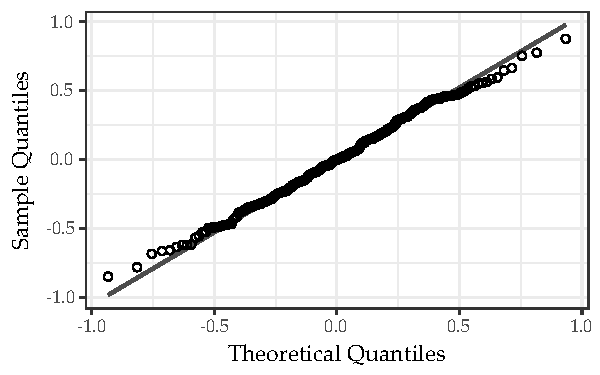
\includegraphics[width=0.45\textwidth]{./images/natl_low_resid_qqplot}
				\label{fig:natl_low_resid_qqplot}%
				}%
			\subfloat[Residuals vs fitted (low SST)]{%
				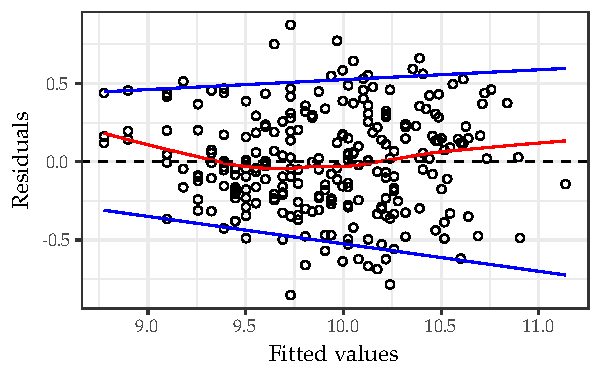
\includegraphics[width=0.45\textwidth]{./images/natl_low_resid_fitted}
				\label{fig:natl_low_resid_fitted}%
				}%
			\caption{Diagnostic plots to analyse the residuals for the North Atlantic basin}
			\label{fig:natl_residuals}
		\end{figure}
	\end{onlyenv}

	\begin{onlyenv}<4>
		\begin{figure}[H]
			\centering
			\subfloat[Q-Q plot (high SST)]{%
				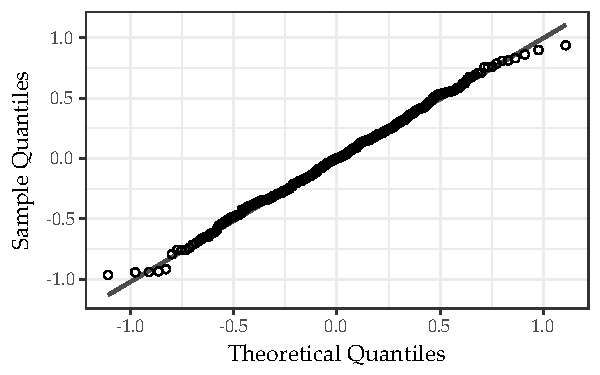
\includegraphics[width=0.45\textwidth]{./images/natl_high_resid_qqplot}
				\label{fig:natl_high_resid_qqplot}%
				}%
			\subfloat[Residuals vs fitted (high SST)]{%
				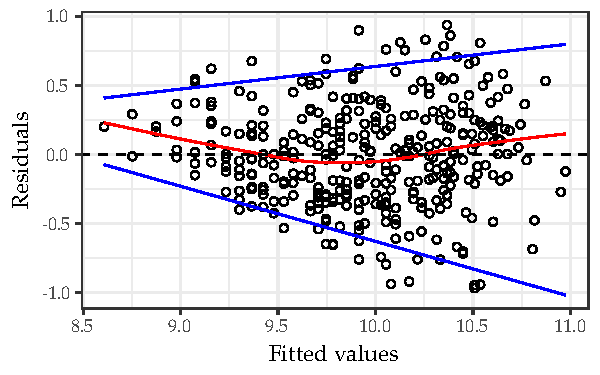
\includegraphics[width=0.45\textwidth]{./images/natl_high_resid_fitted}
				\label{fig:natl_high_resid_fitted}%
				}%
			\caption{Diagnostic plots to analyse the residuals for the North Atlantic basin}
			\label{fig:natl_residuals}
		\end{figure}
	\end{onlyenv}
\end{frame}


%---------------------------------
\subsection{Bootstrapping the coefficients}
\begin{frame}[label=intro-tc]{The bootstrap}
	% \framesubtitle{In plain, example, and \alert{alert} flavour}
	We need a more robust linear model to be able to infer statistical properties of the data using linear regression as the underlying model.

	\medskip
	\footnotesize
	\IncMargin{1em}
	\begin{algorithm}[H]
		\caption{Resampling the cases using bootstrap}
		\label{alg:bootstrap-theory}
		\DontPrintSemicolon
		\For{$r \gets 1$ \KwTo $R$}{
			$\text{(i)}$ Sample $i^{\ast}_{1}, \dots, i^{\ast}_{n}$ randomly with replacement from $\qty{1, 2, \dots, n}$.\;
			\For{$j \gets 1$ \KwTo $n$}{
				$\text{(ii)}$ Set $x_{j}^{\ast} = x_{i^{\ast}_{j}}$, $y_{j}^{\ast} = y_{i^{\ast}_{j}}$ \;
			}
			$\text{(iii)}$ Fit OLS regression to $(x_{i}^{\ast} , y_{i}^{\ast}), \dots , (x_{n}^{\ast} , y_{n}^{\ast})$.\;
			$\text{(iv)}$ Calculate estimates of $\hat{\beta}_{0,r}^{\ast}$ and $\hat{\beta}_{1,r}^{\ast}$.
		}
	\end{algorithm}
	\DecMargin{1em}
\end{frame}

\begin{frame}[label=intro-tc]{Bootstrapping the coefficients}
	% \framesubtitle{In plain, example, and \alert{alert} flavour}
	\begin{figure}[H]
		\centering
		\subfloat[Histogram of the bootstrapped intercept]{%
			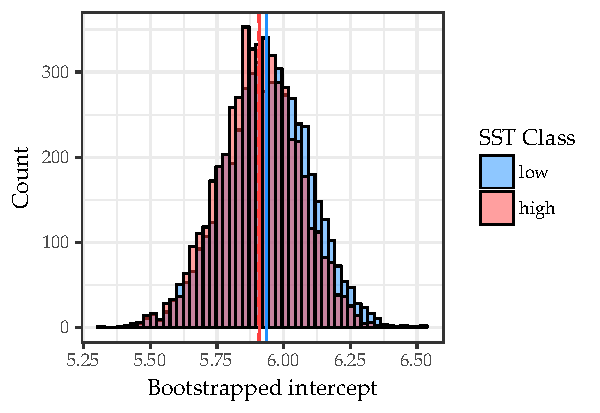
\includegraphics[width=0.45\textwidth]{./images/natl_boot_inter}
			\label{fig:natl-boot-inter}%
			}%
		\subfloat[Histogram of the bootstrapped slope]{%
			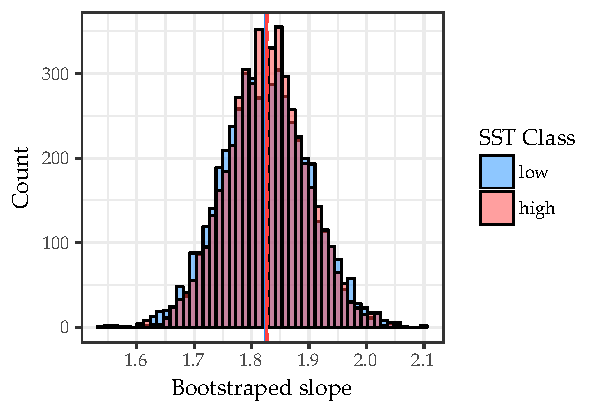
\includegraphics[width=0.45\textwidth]{./images/natl_boot_slope}
			\label{fig:natl-boot-slope}%
			}%
		\caption{Resampled slopes and intercepts obtained by bootstrapping for the North Atlantic basin data for the $PDI(\text{lifetime})$ regression model}
		\label{fig:natl-boot-coefs}
	\end{figure}
\end{frame}

\begin{frame}[label=intro-tc]{Results}
	% \framesubtitle{In plain, example, and \alert{alert} flavour}
	\begin{table}[H]
		\centering
		\resizebox{0.8\textwidth}{!}{%
		\begin{tabular}{cccccc}
			\toprule
			\toprule
			$X$ & $Y$ & SST class & $\hat{\beta}_{0}^{\ast}$ & $\hat{\beta}_{1}^{\ast}$ & $R^{2\ast}$ \\
			\midrule
			\multirow{2}{*}{lifetime} & \multirow{2}{*}{$PDI$}
			 & Low  & \num{ 5.91 \pm 0.17} & \num{1.84 \pm 0.08} & \num{0.67 \pm 0.03} \\
			&& High & \num{ 5.90 \pm 0.15} & \num{1.83 \pm 0.07} & \num{0.61 \pm 0.03} \\
			\midrule
			\multirow{2}{*}{$PDI$} & \multirow{2}{*}{lifetime}
			 & Low  & \num{-1.44 \pm 0.15} & \num{0.36 \pm 0.02} & \num{0.67 \pm 0.03} \\
			&& High & \num{-1.15 \pm 0.14} & \num{0.34 \pm 0.01} & \num{0.62 \pm 0.03} \\
			\bottomrule
		\end{tabular}}
		\caption{Linear regression coefficients obtained performing bootstrap on the North Atlantic basin data}
		\label{tab:natl-boot-coefs}
	\end{table}

	\begin{table}[H]
		\centering
		\resizebox{0.8\textwidth}{!}{%
		\begin{tabular}{cccccccc}
		\toprule
		\toprule
		$X$   & $Y$   & $T^{(1)}$ & $T^{(2)}$ & $T^{(3)}$ & $T^{(4)}$ & $T^{(5)}$ & $T^{(6)}$ \\
		\midrule
		lifetime & $PDI$ & $0.289$ & $0.027$ & $0.048$ & $1.404$ & $1.324$ & $2.727$ \\
		$PDI$ & lifetime & $0.007$ & $0.007$ & $0.054$ & $0.031$ & $0.065$ & $0.095$ \\
		\bottomrule
		\end{tabular}}
		\caption{~Value of the studied statistics for North Atlantic basin data set using bootstrap}
		\label{tab:base-natl-boot-statistics}
	\end{table}
\end{frame}

%---------------------------------
\subsection{Permutation tests}
\begin{frame}[label=intro-hypothesis]{The permutation test}
	We need to properly quantify the statistical significance of evidence against (or in favour of) the hypothesis.
	% \framesubtitle{Formulae, equations, and expressions}

	\medskip
	\footnotesize
	\IncMargin{1em}
	\begin{algorithm}[H]
		\caption{Permutation test for comparing two populations}
		\label{alg:perm-test-theory}
		\DontPrintSemicolon
		$\text{(i)}$ Define the null hypothesis, $H_{0}$, and the alternative.\;
		$\text{(ii)}$ Consider a test statistic that compares the populations which is large (small) if the null hypothesis is not true, and small (large) if it is true.\;
		$\text{(iii)}$ Calculate the true statistic of the data, $T$.\;
		\For{$r \gets 1$ \KwTo $R$}{
			$\text{(iv)}$ Create a new data set consisting of the data, randomly rearranged. Exactly how it is rearranged depends on the null hypothesis.\;
			$\text{(v)}$ Calculate the statistic for this new data set, $T^{\ast}$.\;
			$\text{(vi)}$ Compare the statistic $T^{\ast}$ to the true value, $T$.\;
		}
		$\text{(vii)}$ If the true statistic is greater (lower) than 95\% of the random values, then one can reject the null hypothesis at $p<0.05$.\;
	\end{algorithm}
	\DecMargin{1em}

\end{frame}

\begin{frame}{Results}
	\begin{table}[H]
		\centering
		\resizebox{0.8\textwidth}{!}{%
		\begin{tabular}{cccccccc}
		\toprule
		\toprule
		$X$  & $Y$       & $T^{(1)}$ & $T^{(2)}$ & $T^{(3)}$ & $T^{(4)}$ & $T^{(5)}$ & $T^{(6)}$ \\
		\midrule
		lifetime & $PDI$ & $0.146$   & $0.121$   & $0.711$   & $0.137$   & $0.117$   & $0.128$   \\
		$PDI$ & lifetime & $0.870$   & $0.806$   & $0.705$   & $0.864$   & $0.795$   & $0.830$   \\
		\bottomrule
		\end{tabular}}
		\caption{List of $p$-values of the bootstrap-powered permutation test for the North Atlantic basin data}
		\label{tab:perm-natl-boot-p-vals}
	\end{table}
	This indicates a strong evidence in favour of the null hypothesis being true.
\end{frame}


%-----------------------------------------------------------------
\section{Geographical analysis}
\begin{darkframes}
	\begin{frame}
		\huge Geographical analysis
	\end{frame}
\end{darkframes}

\subsection{New variables}
\begin{frame}{New variables}
	% \framesubtitle{Lewis Carroll}
	We focus on the geographical \textbf{genesis location} of a tropical-cyclone, as well as its \textbf{death location}.

	\medskip
	Additionally, we calculate the total travelled distance, or \textbf{path length}, of each hurricane by means of the \emph{spherical law of cosines}.
\end{frame}

%---------------------------------
\subsection{Analysis}
\begin{frame}{Path length and duration}
	% \framesubtitle{Lewis Carroll}
	\begin{onlyenv}<1>
		We define mean forward speed is calculated as
		\begin{align}
			\ev{v_{f}} = \frac{d}{\text{lifetime}} .
		\end{align}
		We think this variable may be an intermediary variable to relate the storm path length and its $PDI$, and expect a displacement to higher speeds for high-SST years.
	\end{onlyenv}


	% In \Cref{fig:natl-forward-speed} we show a histogram of the mean forward speed for the North Atlantic basin, while in \Cref{fig:epac-forward-speed} we show the same histogram for the Northeast Pacific basin.

	% As it can be seen, there seems to be no general trend on the behaviour of the mean forward between the North Atlantic and Northeast Pacific basins.
	\begin{onlyenv}<2>
		\begin{figure}[H]
			\centering
			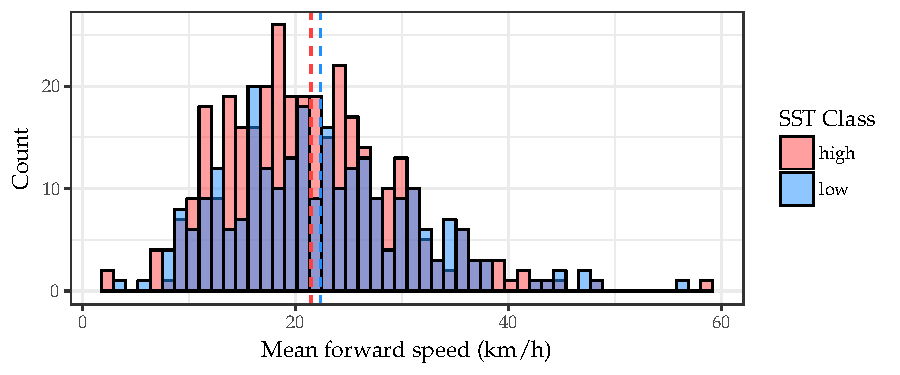
\includegraphics[width=0.6\textwidth]{images/natl-forward-speed}
			\caption{Mean forward speed histogram for the North Atlantic basin}
			\label{fig:natl-forward-speed}
		\end{figure}

		\begin{figure}[H]
			\centering
			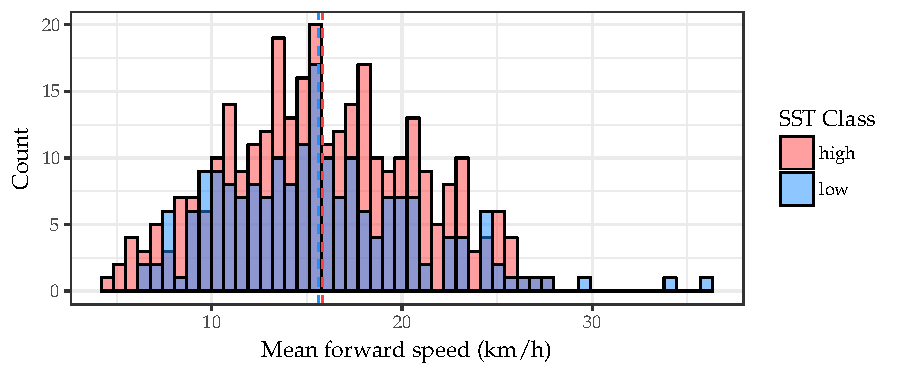
\includegraphics[width=0.6\textwidth]{images/epac-forward-speed}
			\caption{Mean forward speed histogram for the Northeast Pacific basin}
			\label{fig:epac-forward-speed}
		\end{figure}
	\end{onlyenv}

\end{frame}

\begin{frame}{Location}
	% \framesubtitle{Lewis Carroll}
	\begin{onlyenv}<1>
		\begin{figure}[H]
			\centering
			\subfloat[Distribution of the genesis longitude]{%
				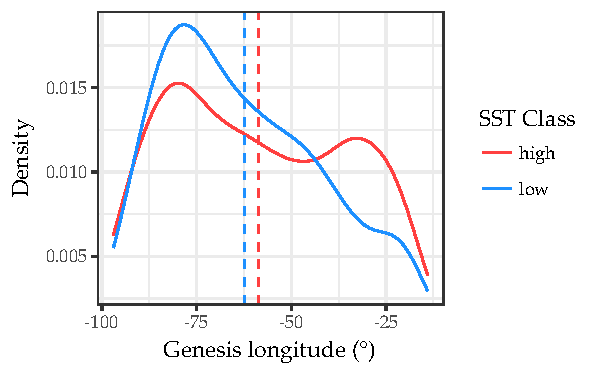
\includegraphics[width=0.5\textwidth]{./images/natl-init-long}
				\label{fig:images/natl-init-long}%
				}%
			\subfloat[Distribution of the death longitude]{%
				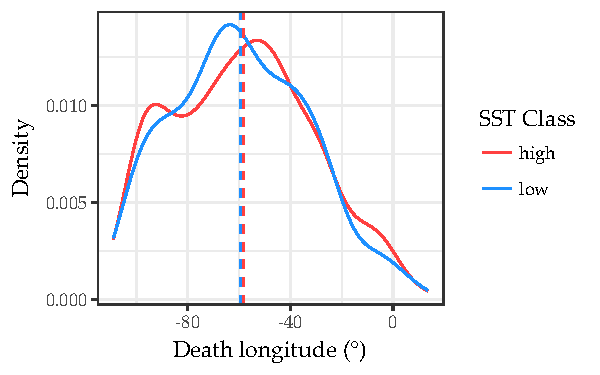
\includegraphics[width=0.5\textwidth]{./images/natl-final-long}
				\label{fig:images/natl-final-long}%
				}%
			\caption{Longitude distributions of storms for the North Atlantic basin}
			\label{fig:natl-positions}
		\end{figure}
	\end{onlyenv}

	\begin{onlyenv}<2>
		\begin{figure}[H]
			\centering
			\subfloat[Distribution of the genesis latitude]{%
				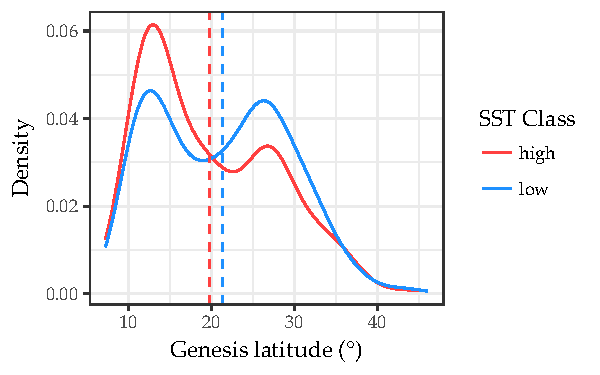
\includegraphics[width=0.5\textwidth]{./images/natl-init-lat}
				\label{fig:images/natl-init-lat}%
				}%
			\subfloat[Distribution of the death latitude]{%
				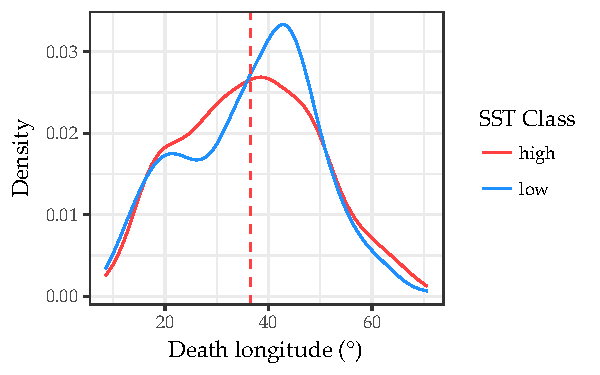
\includegraphics[width=0.5\textwidth]{./images/natl-final-lat}
				\label{fig:images/natl-final-lat}%
				}%
			\caption{Latitude distributions of storms for the North Atlantic basin}
			\label{fig:natl-positions}
		\end{figure}
	\end{onlyenv}

	\begin{onlyenv}<3>
		Major difference between low-SST and high-SST years is the location of the genesis:
		\begin{itemize}
			\item N.~Atl: genesis $\to$ SE, death is not displaced.
			\item E.~Pac: genesis $\to$ SE, death $\to$ NE.
		\end{itemize}
		% The results suggest show the major difference between low-SST and high-SST years is the location of the genesis of the hurricanes, as it seems to be displaced to the South-East. Contrarily to the North Atlantic, in the Northeast Pacific, there seems to be a slight displacement in the death position for high-SST years to the North-East.
	\end{onlyenv}
\end{frame}


%-----------------------------------------------------------------
\section{Conclusions}
% \begin{darkframes}
% 	\begin{frame}
% 		\huge Conclusions
% 	\end{frame}
% \end{darkframes}

% \subsection{Objectives}
\begin{darkframes}
\begin{frame}{Conclusions}
	% \framesubtitle{Lewis Carroll}
	Our conclusions are compatible with the view of tropical cyclones as an activation process, in which, once the event has started, its intensity is kept in critical balance between attenuation and intensification (and so, higher SST does not trigger more intensification).

	\medskip
	Further analysis shows that the longer lifetimes are mainly due to a shift to South-East of the TC genesis point.
\end{frame}
\end{darkframes}

\appendix
\begin{frame}[allowframebreaks]{References}
% \begin{frame}[allowframebreaks]{References}
	\def\newblock{}
	\nocite{Hinkley1997}
	\footnotesize{
	% \nocite{Corral2010}
	% \nocite{Webster2005}
	% \nocite{Emanuel2003}
	\printbibliography[heading=bibintoc]
	}
\end{frame}

%-----------------------------------------------------------------
\section{Questions?}
\begin{darkframes}
	\begin{frame}
		\huge Questions?
	\end{frame}
\end{darkframes}

%-----------------------------------------------------------------
\begin{darkframes}
	\begin{frame}
		\huge Backup slides
	\end{frame}
\end{darkframes}

\begin{frame}
	\begin{figure}[H]
		\centering
		\subfloat[Marginal distribution of the $PDI$]{%
			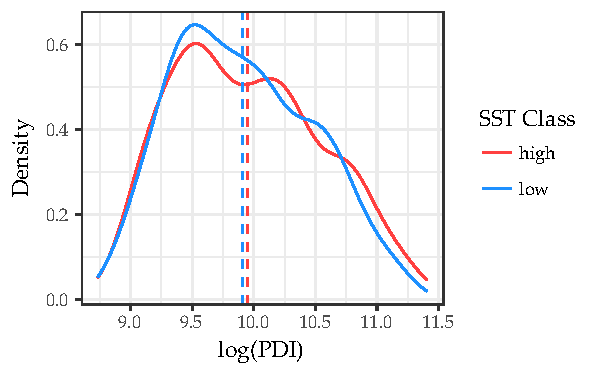
\includegraphics[width=0.5\textwidth]{./images/natl-marginals-pdi}
			\label{fig:natl-marginals-pdi}%
			}%
		\subfloat[Marginal distribution of the lifetime]{%
			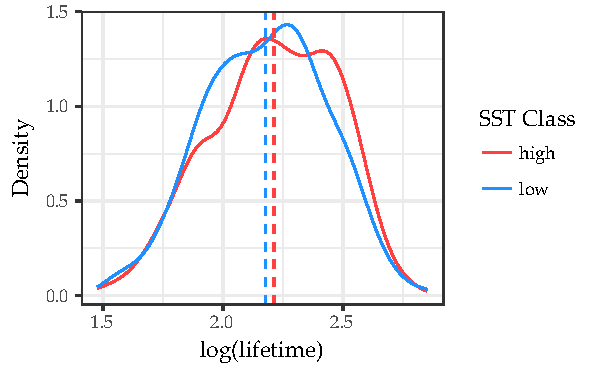
\includegraphics[width=0.5\textwidth]{./images/natl-marginals-lifetime}
			\label{fig:natl-marginals-lifetime}%
			}%
		\caption{Marginal analysis for the variables of the joint distribution for the North Atlantic basin data}
		\label{fig:natl-marginals}
	\end{figure}
	\vspace{-25pt}
	\begin{table}[H]
		\centering
		\resizebox{\textwidth}{!}{%
		\begin{tabular}{ccccc}
			\toprule
			\toprule
			Data & Mean($\log(PDI)$)  & Mean($\log(\text{lifetime})$) & Mean($PDI$) (\SI{e9}{\m\cubed\per\s\squared}) & Mean($\text{lifetime}$) (\si{\hour}) \\
			\midrule
			 Low-SST               & \num{9.91 \pm 0.04} & \num{2.18 \pm 0.02} &
			 \num{22.76 \pm 1.95} & \num{192.94 \pm 5.74} \\
			 High-SST              & \num{9.95 \pm 0.03} & \num{2.21 \pm 0.01} &
			 \num{18.56 \pm 1.74} & \num{176.92 \pm 6.49} \\
			% \midrule
			% % \cmidrule(l){2-5}
			% \multirow{2}{*}{$\log(\text{lifetime})$}
			%  & Low-SST               & \num{2.18 \pm 0.02} & \num{2.19 \pm 0.02} \\
			%  & High-SST              & \num{2.21 \pm 0.01} & \num{2.23 \pm 0.02} \\
			\bottomrule
		\end{tabular}}
		\caption{Statistical summary for the low-SST and high-SST subsets of the marginals distributions for the North Atlantic basin data}
		\label{tab:natl-marginals-stats}
	\end{table}
\end{frame}

\begin{frame}
	\begin{figure}[H]
		\centering
		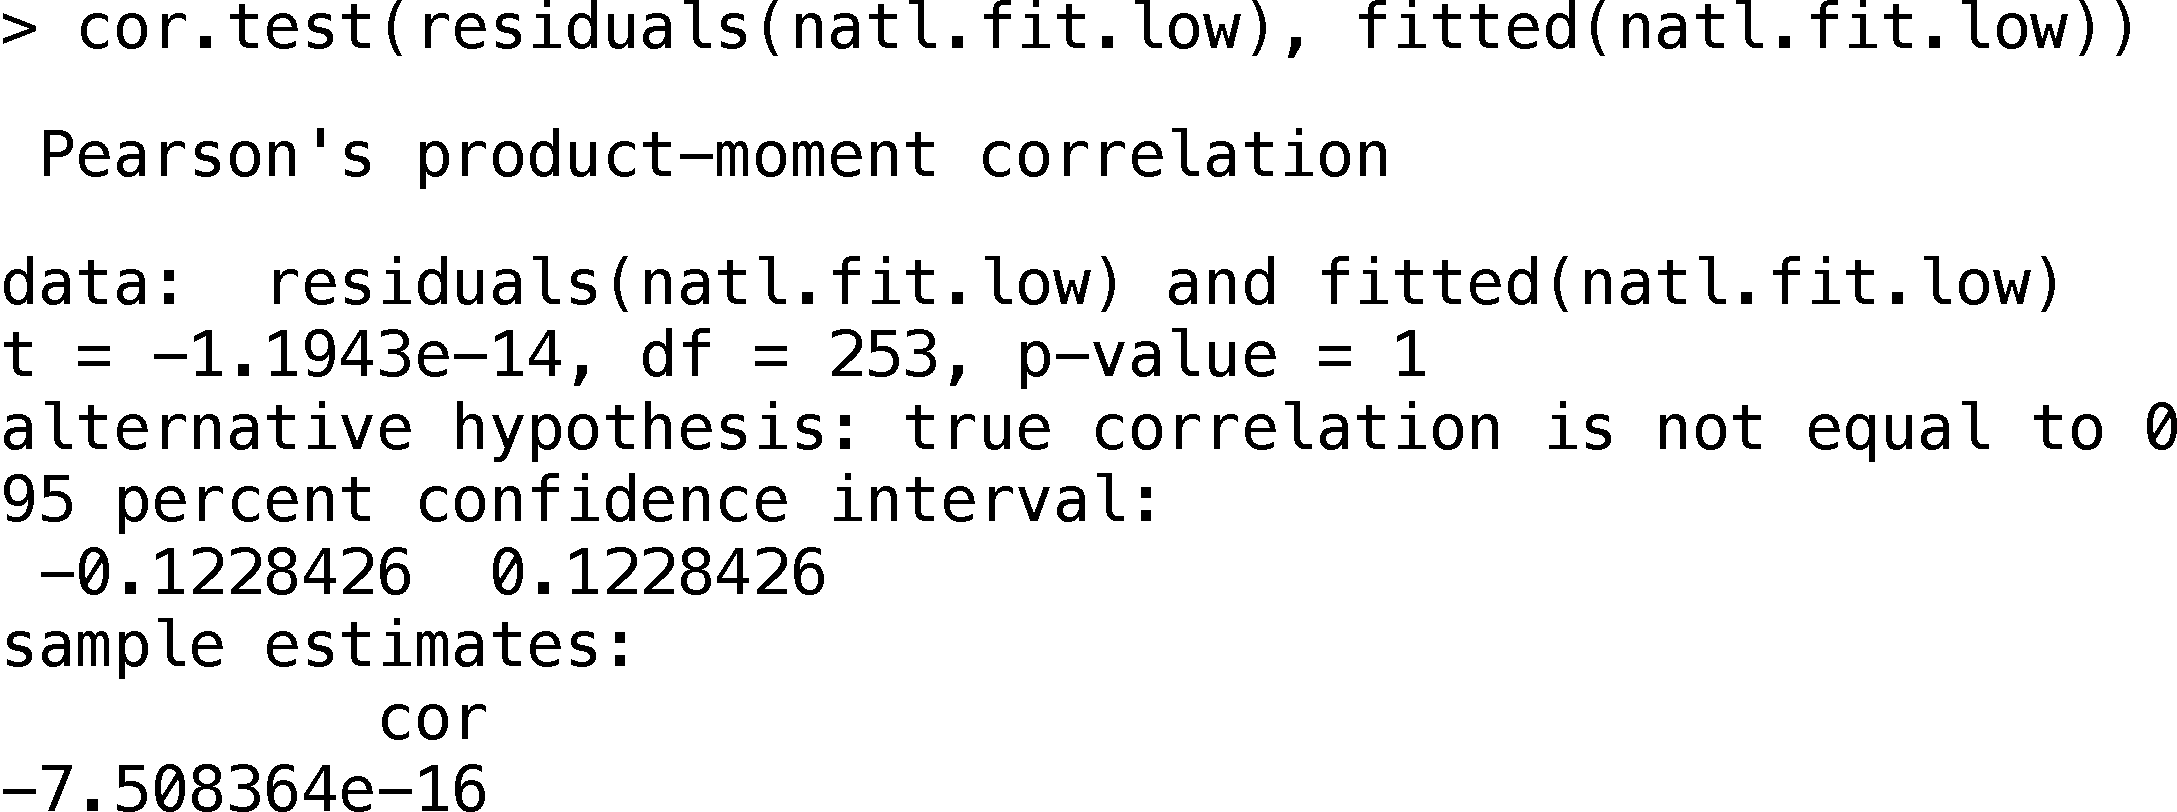
\includegraphics[width=\textwidth]{images/cor-code}
		% \caption{Caption here}
		\label{fig:figure1}
	\end{figure}
\end{frame}
